\section{Introdução}

\subsection{Overview}

\begin{frame}{Overview}
	Reconstrução de espaços utilizando tecnologia Lidar			
\end{frame}


\subsection{State of Art}

\subsubsection{Tecnologias}

\begin{frame}{Visão Estéreo}
				
	\begin{minipage}{0.5\textwidth}
		\begin{itemize}
			\item Mecanismo similar ao funcionamento estéreo do olho humano.
			\item Distância é calculada pelo cálculo da disparidade entre duas imagens. Esta disparidade é depois transformada numa nuvem de pontos.
			\item Não contem informação dimensional absoluta, apenas relativa.
		\end{itemize}
	\end{minipage}%
	\begin{minipage}{0.5\textwidth}
		\begin{figure}
			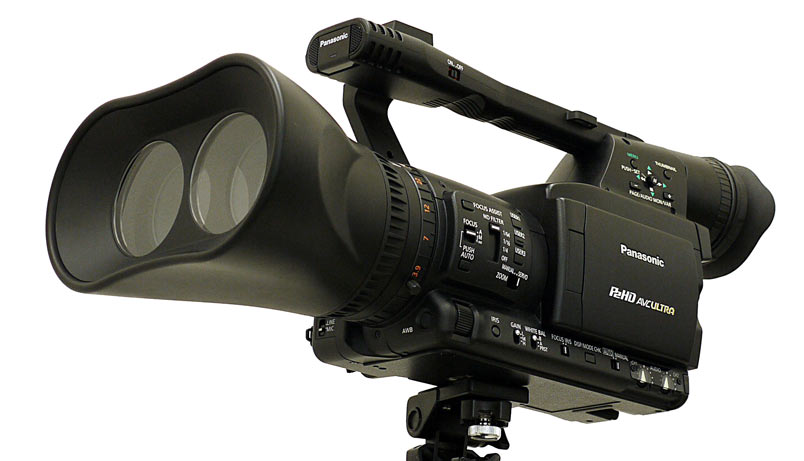
\includegraphics[width=1\textwidth]{img/3d-camera.jpg}
			\caption{Câmara de Vídeo 3d}
		\end{figure}
	\end{minipage}
						
\end{frame}

\begin{frame}{RGBD}
			
	\begin{minipage}{0.5\textwidth}
		\begin{itemize}
			\item Utiliza um sensor destinado à captura da informação de depth. Usualmente é usado uma câmara IR que capta padrões desenhados por um laser.
			\item Resulta numa imagem com informação de cor (RGB) e distância (D).
			\item Esta tecnologia não é muito precisa.
		\end{itemize}
	\end{minipage}%
	\begin{minipage}{0.5\textwidth}
		\begin{figure}
			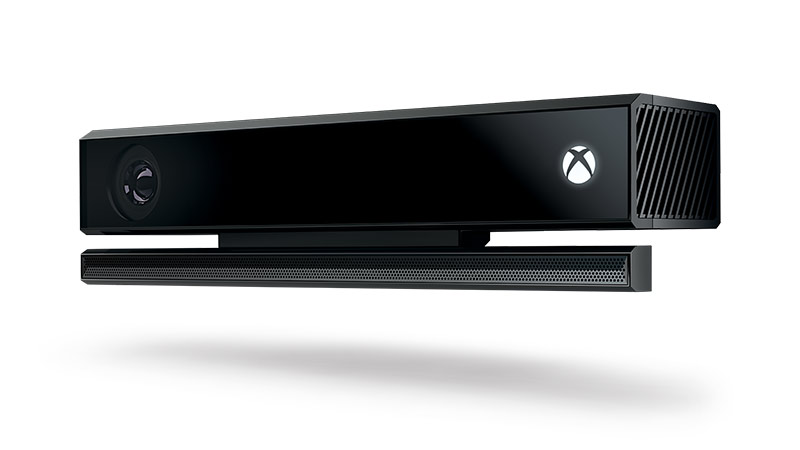
\includegraphics[width=.9\textwidth]{img/kinect.jpg}
			\caption{Kinect}
		\end{figure}
	\end{minipage}
						
\end{frame}

\begin{frame}{Lidar: Light Detection and Ranging}
						
	\begin{minipage}{0.5\textwidth}
		\begin{itemize}
			\item Usa um sinal laser pulsado para medir distancias.
			\item Muito utilizado para medir a topografia da Terra.
			\item Consegue medições muito precisas ($<1mm$).
			\item Não contêm informação de cor.
		\end{itemize}
	\end{minipage}%
	\begin{minipage}{0.5\textwidth}
		\begin{figure}
			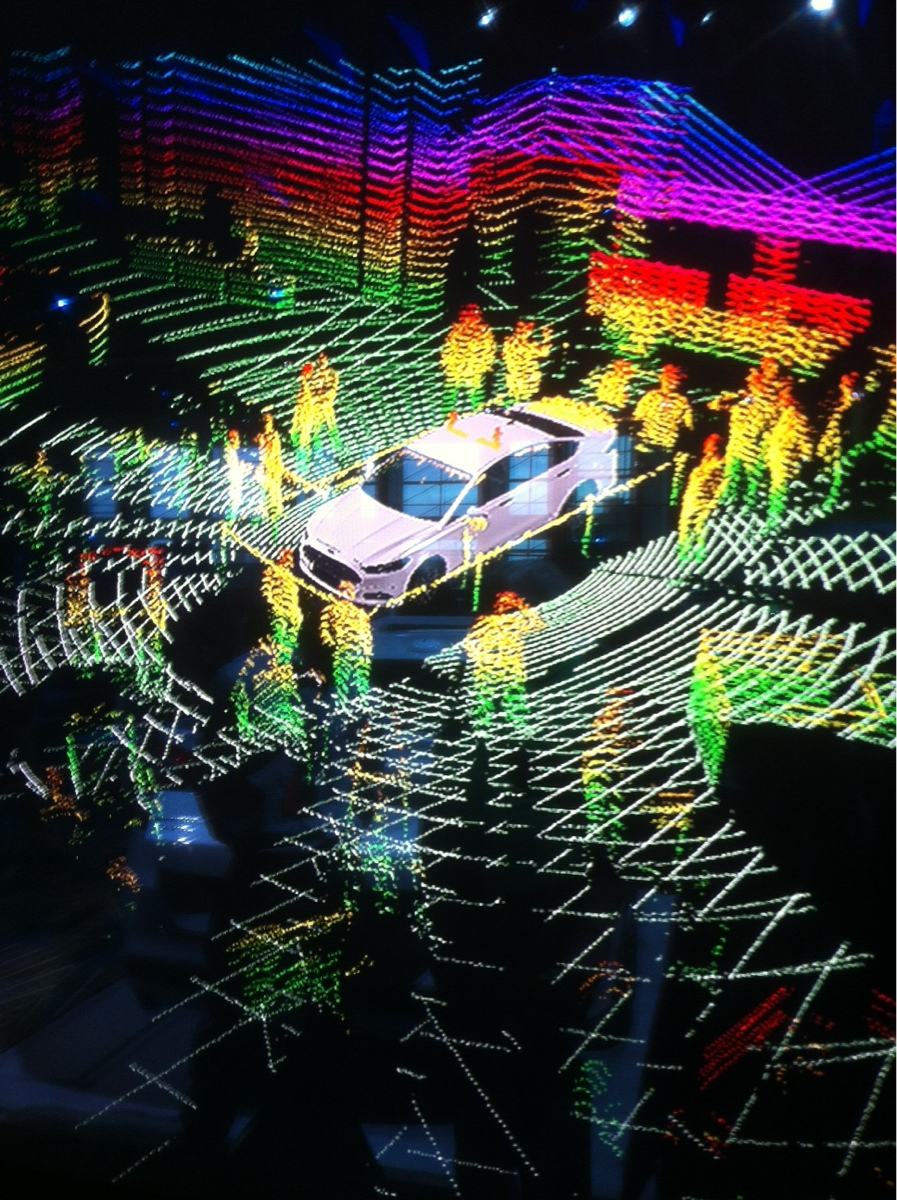
\includegraphics[width=.9\textwidth]{img/lidar.jpg}
			\caption{Nuvem de pontos de um Lidar 3d}
		\end{figure}
	\end{minipage}
																					
\end{frame}

\subsection{Equipamento}

\begin{frame}{Equipamento: Lemonbot}
					
	\begin{minipage}{0.6\textwidth}
		
		\begin{figure}
									
			\begin{tikzpicture}
				\tikzset{
					frame/.style={rectangle, draw=black},
					link/.style={thick}
				}
				\node[frame] (ptu) {PTU};
				\node[frame, below=of ptu] (base) {Base};
				\node[frame, above left=of ptu] (laser) {Laser};
				\node[frame, above right=of ptu] (camera) {Câmara RGB};
													
				\draw[link] (base.north) -| (ptu.south);
				\draw[link] (ptu.west) -| (laser.south);
				\draw[link] (ptu.east) -| (camera.south);
																
			\end{tikzpicture}
									
			\caption{Esquema}
									
		\end{figure}
		
	\end{minipage}%
	\begin{minipage}{.5\textwidth}
		
	\end{minipage}
				
\end{frame}

\begin{frame}{Roadmap}
						    
	\begin{enumerate}
												        
		\item Aquisição da nuvem de pontos 3d. \faCheck
		      		      		      		      		      		      
		\item Calibração extrínseca da Câmara-PTU (hand2eye) e Câmara-Laser (radlocc).
		      		      		      		      		      		      
		\item Triangulação da nuvem de pontos.
		      		      		      		      		      		              
		\item Registo das cores à nuvem de pontos.
		      \begin{itemize}
		      	\item Atribuição da cor a cada vértice (simples).
		      	\item Atribuição da textura à malha (difícil).
		      \end{itemize}
		      		      		      		      		                    
		\item Uniformização da cor entre malhas. Variação é causada por variações nas condições da captura (tempo de exposição/color balance/luminosidade).
		      		      		      		      		      
	\end{enumerate}
						
\end{frame}